\documentclass{article}

\usepackage{amsmath,amsfonts,amssymb,amsthm}
\usepackage{enumerate}
\usepackage{arydshln}
\usepackage{listings,color}
\usepackage{graphicx}

\definecolor{dkgreen}{rgb}{0,0.6,0}
\definecolor{gray}{rgb}{0.5,0.5,0.5}
\definecolor{mauve}{rgb}{0.58,0,0.82}

% Opening
\title{Numerical Analysis HW10\\
Ch21 - 1,2,4 (pg540)\\
Ch22 - 1,8,9 (pg583)\\}
\author{Neal D. Nesbitt}

\begin{document}
\maketitle

\theoremstyle{definition}
\newtheorem{problem}{Problem}[section]
\newtheorem{solution}{Solution}[problem]
\renewcommand*{\thesolution}{\theproblem.\alph{solution}}

\lstset{basicstyle=\ttfamily,
		language=Matlab,
		keywordstyle=\color{blue},
		commentstyle=\color{dkgreen},
		stringstyle=\color{mauve},
		identifierstyle=\bf
		}

\setcounter{section}{20}
\section{}
\begin{problem}
Compute forward and backward difference approximations of $O(h)$ and $O(h^{2})$, and central difference approximations of $O(h^{2})$ and $O(h^{4})$ for the first derivative of $\cos x$ at $x = \pi/4$ using a value of $h=\pi/12$. Estimate the true percent relative error $\varepsilon_{s}$ for each approximation.
\end{problem}

\begin{solution}
Forward difference $O(h)$: \boxed{-0.7911}, $|\varepsilon_{r}| = \boxed{211\%}$
\end{solution}

\begin{solution}
Forward difference $O(h^{2})$:  \boxed{-0.7260} $|\varepsilon_{r}| = \boxed{203\%}$\\
\end{solution}

\begin{solution}
Backward difference $O(h)$: \boxed{-0.6070}, $|\varepsilon_{r}| = \boxed{186\%}$\\\\
\end{solution}

\begin{solution}
Backward difference $O(h^{2})$: \boxed{-0.7197}, $|\varepsilon_{r}| = \boxed{202\%}$\\\\
\end{solution}

\begin{solution}
Central difference $O(h^{2})$:\boxed{-0.6991}, $|\varepsilon_{r}| = \boxed{198\%}$\\\\
\end{solution}

\begin{solution}
Central difference $O(h^{4})$:\boxed{-0.7070}, $|\varepsilon_{r}| = \boxed{200\%}$\\\\
\end{solution}

\begin{problem}
Use centered difference approximations to estimate the first and second derivatives of $y=e^{x}$ at $x=2$ for $h=0.1$. Employ both $O(h^{2})$ and $O(h^{4})$ formulas for your estimates.
\end{problem}

\begin{solution}
First Derivative $O(h^{2})$:\boxed{7.4014}, $|\varepsilon_{r}| = \boxed{0.0017\%}$\\\\
\end{solution}

\begin{solution}
First Derivative $O(h^{4})$:\boxed{7.3890}, $|\varepsilon_{r}| = \boxed{0.000\%}$\\\\
\end{solution}

\begin{solution}
Second Derivative $O(h^{2})$:\boxed{7.3952}, $|\varepsilon_{r}| = \boxed{0.008\%}$\\\\
\end{solution}

\begin{solution}
Second Derivative $O(h^{4})$:\boxed{7.3890}, $|\varepsilon_{r}| = \boxed{0.000\%}$\\\\
\end{solution}

\setcounter{problem}{3}
\begin{problem}
Use Richardson extrapolation to estimate the first derivative of $y=\cos x$ at $x=\pi/4$ using step sizes of $h_{1}=\pi/3$ and $h_{2}=\pi/6$. Employ centered differences of $O(h^{2})$ for the initial estimates.
\end{problem}

\section{}
\begin{problem}
Solve the following initial value problem over the interval from $t=0$ to $2$ where $y(0)=1$. Display all your results on the same graph.
\[ \frac{dy}{dt} = yt^{3} -1.5y \]
\begin{enumerate}[(a)]
\item Analytically
\item Using Euler's method with $h=0.5$ and $0.25$.
\item Using the midpoint method with $h=0.5$.
\item Using the fourth-order RK method with $h=0.5$.
\end{enumerate}
\end{problem}

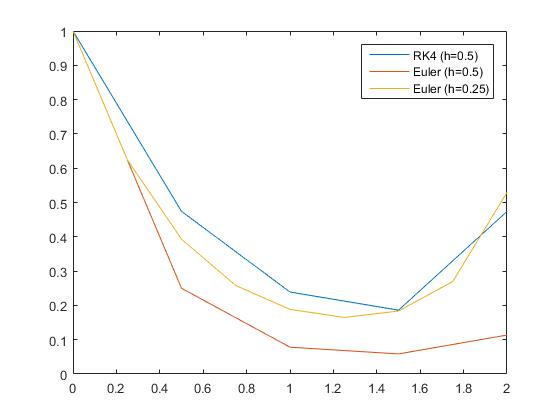
\includegraphics[width=\linewidth]{HW10-ODE1.jpg}

\begin{solution}
Analytically:
\end{solution}

\begin{solution}
Using Euler's method with $h=0.5$ and $0.25$:
\end{solution}

\begin{solution}
Using the midpoint method with $h=0.5$:
\end{solution}

\begin{solution}
Using the fourth-order RK method with $h=0.5$:
\end{solution}

\setcounter{problem}{7}
\begin{problem}
The \textit{van der Pol equation} is a model of an electric circuit that arose back in the days of vacuum tubes:
\[ \frac{d^{2}y}{dt^{2}} -(1-y^{2})\frac{dy}{dt} +y = 0 \]
Given initial conditions, $y(0)=y'(0)=1$, solve this equation from $t=0$ to $10$ using Euler's method with a step size of (a)0.25 and (b) 0.125. Plot both solutions on the same graph.
\end{problem}

\includegraphics[width=\linewidth]{HW10-ODE2.jpg}

\begin{problem}
Given the initial conditions, $y(0)=1$ and $y'(0)=0$, solve the following initial-value problem from $t=0$ to $4$:
\[ \frac{d^{2}y}{dt^{2}} +4y = 0 \]
Obtain your solutions with (a) Euler's method and (b) the fourth-order RK method. In both cases, use a step size of 0.1. Plot both solutions on the same graph along with the exact solution $y=\cos 2t$.
\end{problem}

\includegraphics[width=\linewidth]{HW10-ODE3.jpg}

\end{document}